\chapter{Life-Cycle Energy and Carbon Footprint Modeling with Data Center Building Energy Models}
\label{chp:embodied_cost_model}

\section{Introduction}
    In this chapter, the aim is to quantify the end to end life cycle costs of data centers by extending the operational models developed in the previous chapters. Those operational models have provided an indication of system level energy for a network of data centers and their marginal carbon dioxide footprints. Although, the presented models are a good proxy for the environmental costs of data center operations, they don't account for the energy and carbon footprint embodied in all the materials that the data centers are composed of.

    To assess the end to end environmental impact of data centers, this chapter describes a three-step hybrid life-cycle analysis inclusive of the embodied inventories of the physical data center infrastructure. As the first step, the building energy and marginal costs of energy generation models are reviewed. These two models together provide an indication of the respective costs during the operational phase of a data center's life. Then as the second step, a life cycle modeling framework using an economic input-output (EIO) analysis model extended to environmental costs is introduced. The inputs to the EIO are constructed in this chapter based on literature reviews and the researcher's industrial experience. The final step provides a global view of the end to end assessment by presenting the energy and carbon footprint of each of the data center-language pair analyzed in the previous chapters. With the global view, the global environmental costs of a discrete service can be assessed.

    \subsection{Motivations for an end to end life cycle cost model}
        In terms of scale, US data centers consumed 700 billion kWh in 2016. That was 1.8\% of the total electricity produced in the country according to a United States Department of Energy (DOE) report \cite{Shehabi16}. To drive further intuition of their scale, a typical 100-MW data center at peak load consumes the same amount of energy in an hour as 100 homes do in a month. Given a data centers power demands, it is not surprising that operational energy use has a high sensitivity towards their total cost of ownership (TCO); making it a key metric in TCO based design decisions. While optimization for use phase energy may significantly reduce the carbon footprint of a data center (given the source energy mix does not change), it does not account for other phases in the data center's end to end life cycle. Inventories from embodied life cycle phases such materialization, transit, maintenance, and end of life are left out of the operational phase energy models that have become prevalent indicator of data center sustainability. 

        There are two predominant paradigms for evaluating the embodied environmental inventories for any product that has been altered by technology (techno-sphere). The first method is process based. The complexity of a process-based model is greatly influenced by the boundary conditions of the study. If the boundary is demarcated between the biosphere and the techno-sphere, then the number of distinct life cycle processes to quantify explodes by 500 times for a simple pen \cite{shah11}. The alternate method is based on Leontief's macro-economic proxies that exploits economic correlations between industrial sectors. In macro-economic models, a matrix with rows and columns equal to the number of sectors in the economy is populated with the cost relationship between the row-sector and the corresponding column-sector. Industrial-sector macro-economic proxies reduce the problem space significantly as only one cost vector is required as input to analyze an entire economy. This research combines the two paradigms and presents a hybrid life-cycle assessment model of data centers that can be used to support data center design decisions. 

        The structure of the paper is as follows. First, some technical background about data centers is provided along with a synthesis of similar works. Then in the methodology section a dynamic model to quantify the operational and embodied costs of data center infrastructure is described. The results from the methods as then presented in the results section. This article concludes by summarizing its findings and suggesting the future direction in this area of research. 

\section{Background}
    \subsection{Technical Overview of Data Centers}
        Modern internet data centers are district scale systems, spanning campuses that are hundreds of acres. They may contain several hundred thousand pieces of information technology (IT) equipment. IT equipment consists of physical servers, network hardware nodes, and digital storage media. Theses pieces of IT equipment sit alongside the data center's district scale cooling and electrical distribution plants housed in warehouse-scale built environments. The environmental footprint of a data center spans the full breadth of these physical pieces of infrastructure. 

        At their scale data centers receive power through medium voltage connections with the local utility's grid. The alternating-current voltage may then be stepped down in several steps, but ultimately, it is rectified to be used by the sensitive electronic components in the information technology hardware. Each step-down is a point of power inefficiency, with the alternating-current to direct-current conversion being the biggest point of power loss. Furthermore, anywhere that the step down or conversion occurs inside the building, the electrical inefficiencies are manifested as heat.  

        The heat from the electrical inefficiencies, along with the heat emitted by the IT equipment transistor state transitions and their current leakage, must be rejected to the outside of the building space by mechanical means. At a fundamental level, a mechanically driven fluid mover is needed to convey the heat from indoors to outdoors or another reservoir. In single pass cooling systems fans intake outside-air and force them through the IT equipment, capturing any heat and carrying it outside of the buildings. More complex cooling systems may include liquid or gas refrigerant medium thermodynamic cycles between the buildings and reservoirs, with the refrigerant medium capturing heat at either the building room level or at the scale of IT equipment. Precise modeling of such data center building systems with intense therm-power dynamics is now a manageable task in building energy modeling software \cite{kumar20,kumar20b}. 

        The embodied costs of IT equipment and building systems yield additional environmental costs for a data center's life cycle. The rate of innovation for IT equipment and the ever-increasing demands from the software applications creates a capital market where TCO of one generation of IT hardware rapidly increases relative to newer IT hardware solutions. The capital of cost/performance trade-off makes the positive TCO life of IT equipment between two to five years as observed by Shehabi in the DOE report \cite{Shehabi16}. This relatively short lifetime of IT further compounds the embodied costs of data centers. For example, through a 20-year data center building life, four to ten generations of IT transit through the facility. Disparities in lifetimes and dimensional scale differences between buildings and microchips make data center embodied inventory modeling complex. However, recently hybrid life cycle assessment models have shown to be effective in quantifying the embodied costs of data centers \cite{shah11, whitehead15}. 

        Information technology equipment requires some further insights in order to make its impact to data center life cycle analysis more concrete and directed in scope. At the heart of information technology equipment are microprocessor chips. Modern chips are composed of billions of transistors which have been getting smaller in size since their first applications in electronics signal processing in the 1960's. Transistors have been the key enabler for the compaction and power efficiency gains of electronic devices over the years and they've also been shown to have one of the most dominant environmental costs within electronic products \cite{boyd09, alcaraz18}.

        Prior to the mid-2010's, transistors were composed of planar or 2-D architectures. 2-D transistors inherently had limited operational power efficiencies due to higher voltage and current leakage compared to the novel 3-D processors in the market today. Specifically it's the 3-D processes that have allowed significant operational efficiency gains for data centered operators, yet studies assessing the 3-D transistor architecture's impact to data center life cycle costs are lacking. The 2-D to 3-D transition is a recent example of rapid rate of adaption for information technology equipment that make generalized environmental impacts studies for transducer technology obsolete in two to three years \cite{murphy03}. The frequent churn of technology also drives rapid changes in the manufacturing process of the chips. These rapid changes in semiconductor-manufacturing processes necessitates a parametrically scalable framework where transistor chips can be evaluated in isolation from other server components.  

    \subsection{Similar Works}
        In this section similar works that have quantified the environmental foot print of data centers are presented. Data center life cycle assessment works come from industrial operators \cite{shah11},  academia \cite{whitehead15,kline16}, federal agencies \cite{CLEER13}, and industrial consortium's \cite{tgg12}. Two of the reviewed works are conducive to replicate from the ground up \cite{shah11,whitehead15}, while another serves as a guideline \cite{tgg12}, and another provides an online interactive tool to assess the footprint of targeted classes of Cloud services \cite{CLEER13}. 

        From the operators perspective Shah, demonstrates an end to end life cycle assessment of data center systems \cite{shah11}. Shah uses a hybrid model inclusive of process based and economic input/output assessment frameworks to assess a single a data center, while using a static model for use-phase power. Whitehead, extends Shah's hybrid work and demonstrates the life-cycle costs of a real data center and sets an explicit functional unit of 1-kW of provisioned capacity \cite{whitehead15}.  
        
        The recent focus on product operational energy efficiency motivated Kline’s study of the trade-offs between operational energy and the embodied costs of information technology equipment \cite{kline16}. Although their bases for the embodied costs are process based, their literature does not provide sufficient insight for others to reproduce the work. Similarly, The Green Grid's Data Center Life Cycle costs guidelines outline the end goal of a data center life cycle analysis. It classifies several key attributes that need to be considered, but lacks references to explicit procedures that must be followed to achieve the goals. 
        
       The Cloud Energy and Emissions Research (CLEER) Model provides a browser based user interface to compare the environmental costs of on-premise server based services with hypothetical cloud-based systems that would provide an equivalent service \cite{CLEER13}. CLEER's analysis is transparent and inclusive of embodied and operational costs, but it does not dynamically couple the embodied or operational costs into the model. The presented set of past works has inspired the methodology of this research as described in the next section.

\section{Methodology}
    \subsection{Functional Unit and Reference Flows}
    Life cycle assessment studies require a functional unit of performance of the system under study for use as a normalized reference point. As a reference point for data centers, there is an industry wide consensus that power is the best indicator for a data center's workload capacity \cite{shah11, whitehead15, barroso18}. Based on the consensus, the functional unit adapted for this research is chosen to be 1-kW of provisioned power per year. 
    
    Furthermore, for the abstracted functional unit to be used in comparisons between different data center design scenarios requires it to be translated to reference flow values. In this work the reference flow is constrained to 1-year of data center operations with the globally provisioned power footprint of each of the language abstracted internet services. The language (internet service) to data center distribution is indicated in Figure~\ref{land_dc_sankey}. 
    
    \begin{figure}[h!]\centering
    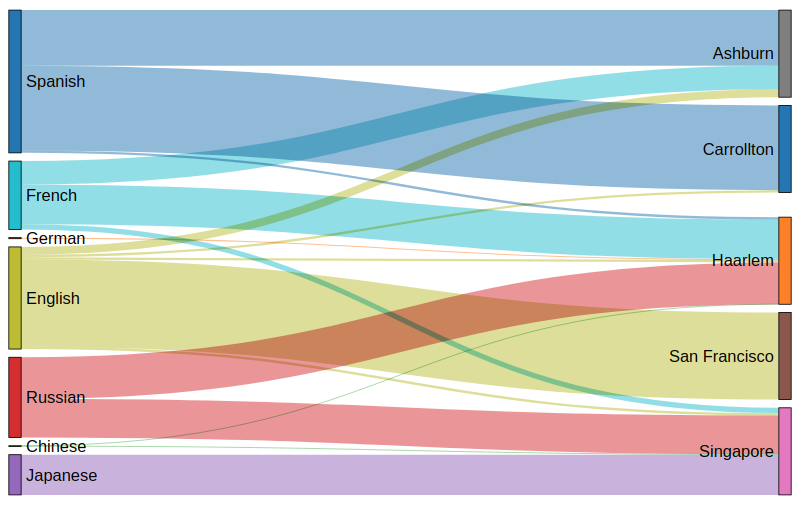
\includegraphics[scale=0.4]{embodied_cost_model/images/lang_dc_sankey.png}
    \caption[Language to Data Center Site Sankey Diagram]{Language to data center flows. The thickness of the links at each data center site indicate the relative portion of traffic that the respective language demands at the data center.}
    \label{land_dc_sankey}
    \end{figure}
    
    \subsection{System Boundary}
    The presented framework is intended to be used as a tool in data center life cycle assessments (LCA), where prevalent LCA practices are followed. In standard practice, product specific LCA studies generally entail four phases: 1) goal and scope phase, 2) the inventory analysis phase, 3) the impact assessment phase, and 4) the interpretation phase \cite{ISO14040}. The methodology, data sets, and software tools presented in the research is conducive for the first three LCA phases which all require quantitative assessment of data center environmental footprints. Stated more explicitly, this research’s goal is to provide a model that can be used to quantify the energy and carbon footprint of data center systems encompassing the embodied and operational phases in a single workflow. 
    
    Figure~\ref{system_boundary} illustrates the boundary conditions the boundary conditions with in the scope of this framework. In the scope are for paths of input of raw materials and energy from the ecosphere. Two paths lead to the embodied systems found in data centers; building construction and information technology manufacturing. While the other two path lead to the operational systems that are required to run the data centers. 
    
    \begin{figure}[h!]\centering
    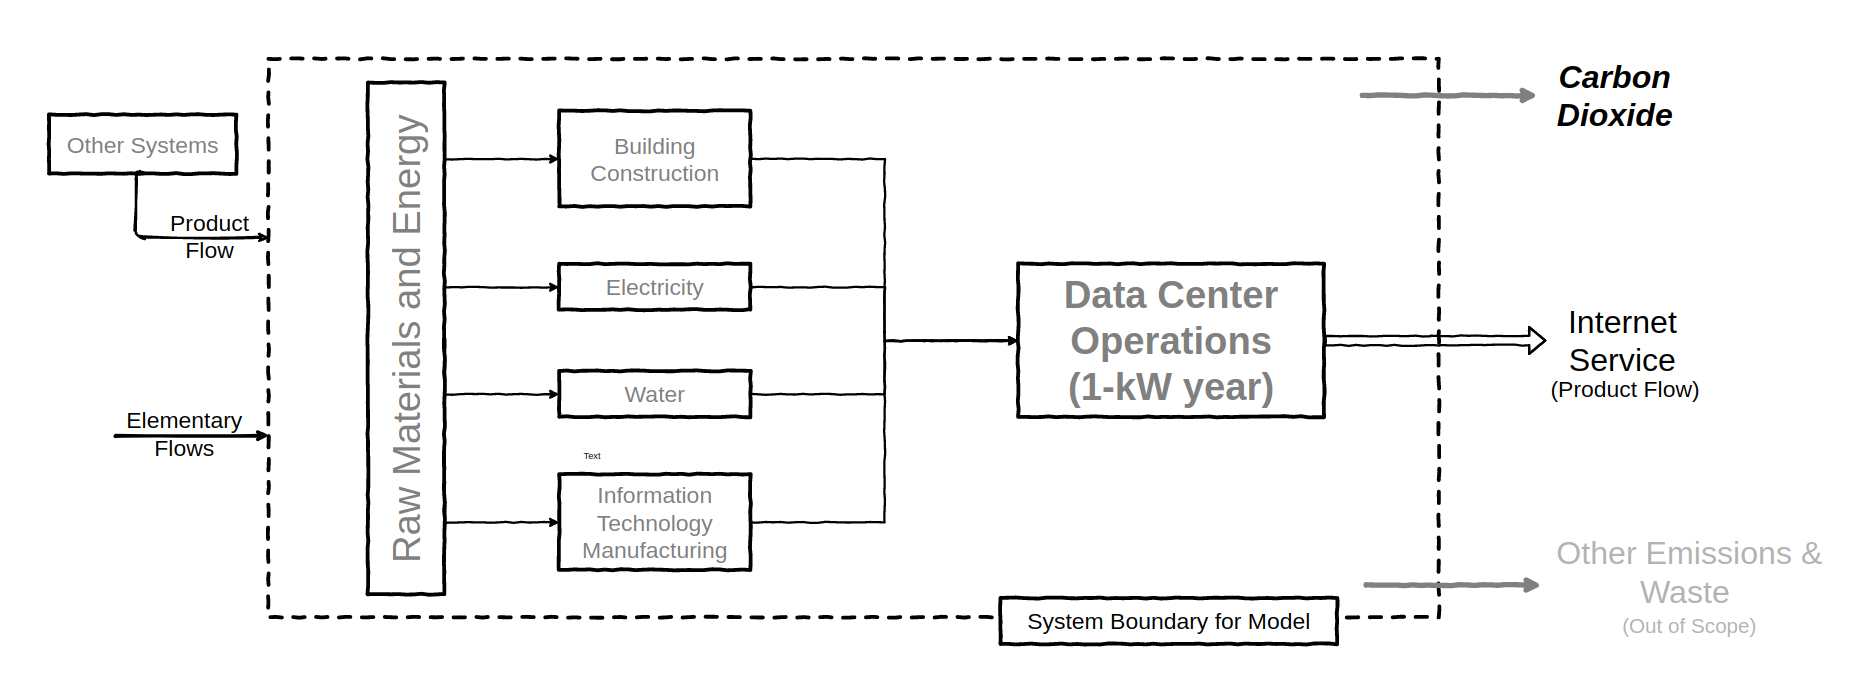
\includegraphics[scale=0.25]{embodied_cost_model/images/system_boundary2.png}
    \caption[System Boundary Diagram]{System Boundary for 1-kW of Provisioned Data Center Capacity.}
    \label{system_boundary}
    \end{figure}
    
    In this research specific sub-systems of data centers are segregated as listed in Table~\ref{tab:dc_subsystem_boundaries}. Demarcation by these boundaries allows development of the embodied and operational models to align with industrial cost data and in terms of EIO industrial vectors. Table~\ref{tab:dc_subsystem_boundaries} serves the structural backbone for all the models developed in this framework as discussed next.
    
    \begin{table}[h]
\centering
\begin{tabular}{|l|l|} \hline
\bf{System Boundary} & \bf{Examples} \\ \hline 
Building Systems & Data Center Shell and Core \\ \hline
Cooling Systems & Air Handling Units and hydronic plants \\ \hline
Power Distribution & UPS, PDU, Cables, Diesel Generators \\ \hline
Information Technology & Compute, Storage, Network \\
\hline\end{tabular}
\caption{Sub System Boundaries}
\label{tab:dc_subsystem_boundaries}
\end{table}
    
    \subsection{Operational Inventories}
    
    \comment{The functional unit is not tied with the operational energy. The result maybe something like $\frac{kWh}{kw}$ (?) the lower the the number the more adverse it will be. Also this can be relative factor; i.e 1 for kWh*8760 hours, with kWh - kW capacity.}
    
    There are extensive theoretical data center power use models in literature \cite{dayarathna16, joshi12}. However, industrial power usage insights are lacking in the public domain \cite{Masanet20}. As an exception some industrial insights are provided by Barroso in \cite{barroso18, barroso13}. Barroso provides Google's distribution of power for various points-of-use as indicted by the pie-charts shown in Figure~\ref{power_2012} and Figure~\ref{power_2017} for two generations of technology. In 2012, more than 80\% of the energy in a data center was used by four components; CPU 42\%, Cooling 15.4\%, disk 14.3\% and DRAM 11.7\%. By 2017, the cooling overhead had decreased to only account for 3\% a data center energy use, this decrease in cooling inflated the relative fraction of CPU and DRAM energy requirement. From these distributions, it is apparent that CPU's power usage is the dominant hot-spot.  
    
    The values in Figure~\ref{power_2012} and Figure~\ref{power_2017} are annualized distributions. In practice the power demand of data centers is very dynamic and sensitive to complex workload dependencies. These dependencies lend themselves to be exploited in power proportional computing paradigms. Several proportional workload techniques are discussed in detail by O'Sullivan in \cite{osullivan15}. This research takes such techniques and extends building energy models to be aware of proportional CPU loads based on coming network traffic to a data center site.
    
    \definecolor{pistachio}{rgb}{0.58, 0.77, 0.45} %cpu
\definecolor{denim}{rgb}{0.08, 0.38, 0.74} %dram
\definecolor{babyblue}{rgb}{0.54, 0.81, 0.94} % disk/hdd
\definecolor{azure}{rgb}{0.0, 0.5, 1.0} % storage
\definecolor{chartreuse}{rgb}{0.5, 1.0, 0.0} % nw
\definecolor{ashgrey}{rgb}{0.7, 0.75, 0.71} % balance/misc
\definecolor{bananamania}{rgb}{0.98, 0.91, 0.71} % psu
\definecolor{citrine}{rgb}{0.89, 0.82, 0.04} % power dist
\definecolor{cinnabar}{rgb}{0.89, 0.26, 0.2} %cooling

\begin{figure}[h]
\centering

\begin{tikzpicture}

% specify the pie charts
\node [anchor=center] (mix-ssd) at (0,3.5) {Power Allocation in 2012 \cite{barroso13}};
\pie[explode={0, 0, 0, 0}, , radius = 3, text=hide,color={pistachio, denim, babyblue, chartreuse, ashgrey, citrine, cinnabar }] 
{42/cpu, 11.7/dram, 14.3/disk, 4.9/nw, 4/misc, 7.7/power_dist, 15.4/cooling}
\definecolor{airforceblue}{rgb}{0.36, 0.54, 0.66}
\node [anchor=center] (mix-hdd) at (7,3.5) {Power Allocation in 2017 \cite{barroso18}};
\pie[pos={7,0}, explode = 0, radius = 3, text=hide, color={pistachio, denim, azure, chartreuse, ashgrey, citrine, cinnabar }] {60.6/cpu, 17.9/dram, 2.0/storage, 5.0/nw, 4/misc, 7.6/power_dist, 3.0/cooling}

%Specify the legend
\node [anchor=east] (cpu) at (-2,-3.8) {\small{CPU}};
\filldraw[outer color=pistachio, inner color=pistachio] (-2,-4) rectangle (-1.6,-3.6); % cpu

\node [anchor=east] (storage) at (0,-3.8) {\small{DRAM}};
\filldraw[outer color=denim, inner color=denim] (0,-4) rectangle (0.4,-3.6); % dram

\node [anchor=east] (disk) at (1.8,-3.8) {\small{Disk}};
\filldraw[outer color=babyblue, inner color=babyblue] (1.8,-4) rectangle (2.2,-3.6); % disk

\node [anchor=east] (psu) at (4,-3.8) {\small{Storage}};
\filldraw[outer color=azure, inner color=azure] (4,-4) rectangle (4.4,-3.6); %nw

\node [anchor=east] (balance) at (6.2,-3.8) {\small{Balance}};
\filldraw[outer color=ashgrey, inner color=ashgrey] (6.2,-4) rectangle (6.6,-3.6); % balance

\node [anchor=east] (power) at (10,-3.8) {\small{Power Distribution}};
\filldraw[outer color=citrine, inner color=citrine] (10,-4) rectangle (10.4,-3.6); % power dist

\node [anchor=east] (cooling) at (2,-4.6) {\small{Cooling}};
\filldraw[outer color=cinnabar, inner color=cinnabar] (2,-4.8) rectangle (2.4,-4.4); %cooling

\node [anchor=east] (nw) at (6,-4.6) {\small{Network}};
\filldraw[outer color=chartreuse, inner color=chartreuse] (6,-4.8) rectangle (6.4,-4.4); %nw

\end{tikzpicture}

\caption[Barroso's Power Distribution]{Data Center Power Distribution for Two Generation of Technology}
\label{fig:power_dist_pies}
\end{figure}
    
    Specifically, the embodied costs of the data center materials are extended to the EnergyPlus model from Chapter~\ref{chp:bem}. EnergyPlus provides a comprehensive indication of the operational energy and together with the marginal cost of energy model from Chapter~\ref{chp:mec}, it exposes the carbon footprint for each of the five data centers and the language abstracted service pairs. Both models are based on the traffic simulator from Chapter~\ref{chp:traffic}. The general framework is illustrated in Figure~\ref{process_flow}.
    
    \begin{figure}[h]
\centering
\begin{tikzpicture}
% \node [anchor=west] (scope) at (8.75,5.5) {Embodied Costs};
\node [anchor=west] (embodied) at (9.6,-.3) {(Scope of Chapter)};
% \node [anchor=west] (traffic) at (1.4,5.5) {Traffic};
% \node [anchor=west] (bem) at (4.2,5.5) {BEM};
% \node [anchor=west] (mec) at (6.75,5.5) {MEC};
\begin{scope}[xshift=1.5cm]
    \node[anchor=south west,inner sep=0] (image) at (0,0) {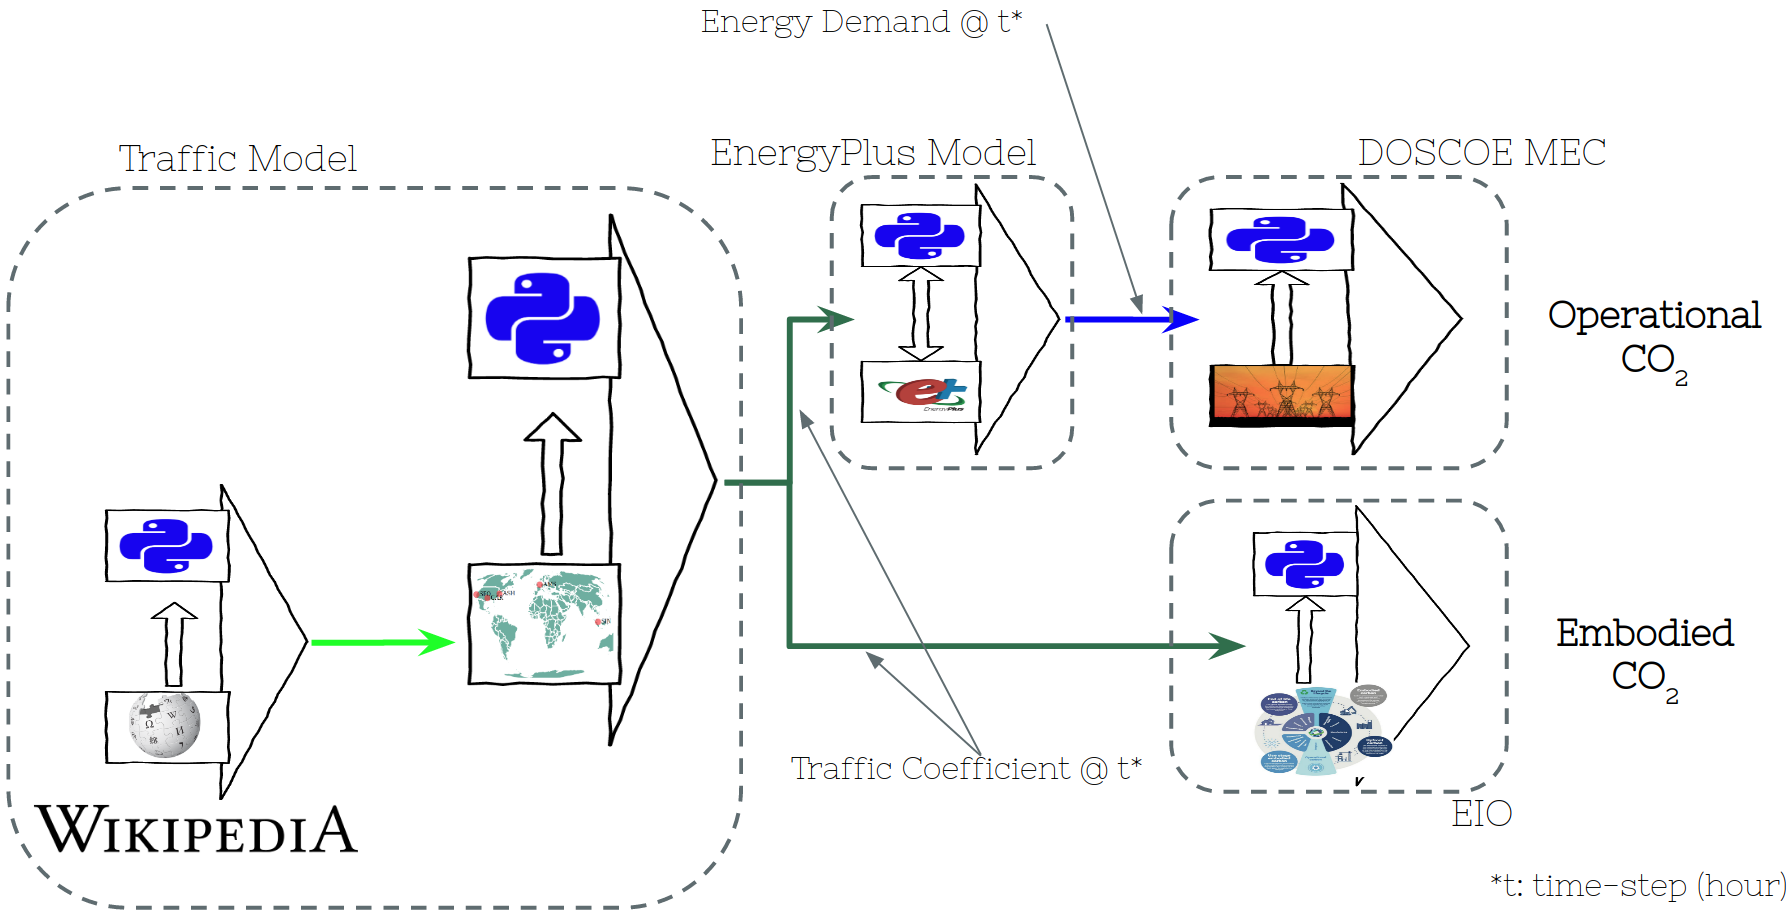
\includegraphics[width=0.8\textwidth]{embodied_cost_model/images/horizontal_process_flow2.png}};
    \begin{scope}[x={(image.south east)},y={(image.north west)}]
        \draw[ultra thick,rounded corners, ,dashed] (0.625,0.90) rectangle (1.05,0..08);
        % \draw [-stealth, line width=5pt, cyan] (scope) -- ++(0.6,0.0);
    \end{scope}
\end{scope}
\end{tikzpicture}
\caption[Model Process Flow Diagram]{Model Process Flow Diagram.}
\label{process_flow}
\end{figure}
    
    \subsection{Embodied Inventories}
    Embodied cost assessments account for the natural resources consumed when extracting, transforming, manufacturing, transporting, constructing, maintaining, and disposing the product under study. The first step in these assessments is to set the boundary conditions of the system. The second step is to select the method of the assessment. Two methods are available for such assessment; namely process based or EIO based. Process based methods are bottoms up procedures; accounting for all processes that are required to transform raw materials into consumer goods. However in process based methods as the product boundary and the count of processes to quantify can have exponentially correlations. This exponential growth can become an intractable task for building designers. A more tractable method is the EIO, where economic relationships between two industries at the national level are exploited. . 
    
    Leontief's original use case of the EIO was to identify the contribution from all economic sectors required to produce a unit of specific products in an economy.  The formulation of Leontief's EIO is indicated by Equation~\ref{eq:Leontief_IO}; where $Y$ is the input costs, $I$ is the identity matrix, and $A$ is the direct costs array \cite{matthews15}. In general direct costs represent the entire economy as a two-dimensional square array, where the rows and columns indicate distinct sectors within the economy. The values in the array indicate the row-index-sector’s input into the column-header-sector. Since their development in the 1930's, EIOs have been commonly used to characterize national economic accounts. More recently, Matthews and Hendrickson showed that EIO can be used for environmental life cycle assessments as-well \cite{matthews15}.  
    
        \begin{equation} \label{eq:Leontief_IO}
        [I-A]^{-1}Y
        \end{equation}
   
    Due to the streamlined approach of the EIO method compared to process based environmental assessments methods, the former is preferred for this research. Specifically, the United States Environmentally Extended Input-Out (USEEIO) model developed by Yang for the EPA is used in this research \cite{yang17}. The USEEIO’s economic relationship between sectors is based on 2007 cost data, while the environmental data are derived from 2013 emissions data. Both were the most up-to-date data available to the researchers at their time of publication. They suggest using 2013 cost of money for inputs, having demonstrated that the underlying structure of the economy has not shifted significantly between 2007 and 2013. 
    
        \subsubsection{Building Systems}
        Typically, data center shells and structural cores are under the jurisdiction of the same building codes as other commercial buildings, i.e. Type IIA construction types. However, the dense population of computers along with the  power and cooling requirements of data centers make several things clearly distinguishable from most commercial building types. The differences are significant enough to make the generic building sector's USEEIO environmental inventories invalid for data centers. 
        
        To more accurately represent data center buildings, several general contractor proposals for new data center construction and retrofit projects were reviewed for the cost distribution of the trades labor and equipment costs.  The contractor cost allocations per trade divisions were then compared with the values of the handful of building construction sectors available in the USEEIO. Based on the comparisons, the USEEIO manufacturing buildings sector is found to be the most similar for data centers. However, there are still shortfalls between data centers and the manufacturing buildings sector. To overcome the shortfalls, a hybrid method was used to construct a more representative Y vector for data centers. 
        
        The resulting Y vector for the building and building utilities systems is shown in Table~\ref{tab:eeio_y_building_table}. The table indicates the cost input required to provision a functional unit of 1 kW of data center capacity. Each sector's cost is derived from the contractor costs for the corresponding construction specification division as listed  in their proposals. Seven explicit sectors are quantified in addition to the manufacturing building sector. The manufacturing building/us is a catch all sector. This sector catches all the building trades that are not represented by the other entries in the Y vector; such as concrete or steel. 
        
        \begin{table}[h]
\centering
\begin{tabular}{|l|l|l|} \hline

\bf{ID} & \bf{Sector Name} & \bf{\$/kW}  \\ \hline

333415 & air conditioning, refrigeration, and heating equipment/us & 550 \\ \hline
333611 & turbines and turbine generator sets/us & 770 \\ \hline
335311 & specialty transformers/us & 50 \\ \hline
335313 & switchgear and switchboards/us & 100 \\ \hline
335920 & communication and energy wire and cable/us & 100 \\ \hline
335999 & other miscellaneous electrical equipment and components/us & 40 \\ \hline
335314 & relay and industrial controls/us & 150 \\ \hline
233230 & manufacturing buildings/us & 5250 \\ \hline

\end{tabular}
\caption{EEIO Costs Vector for Building and Utilities Infrastructure}
\label{tab:eeio_y_building_table}
\end{table}


        
        \subsubsection{Information Technology Systems}
        
        In this subsection the IT equipment's inventories are assessed. The IT equipment in a data center can be categorized broadly into three segments: compute, storage, and network. Within each of these segments, data center operators can further tune the hardware configurations to optimize their workloads. Figure~\ref{fig:server_cost_apportionment} indicates component wise cost distribution for five hardware stock-keeping units (SKU). The SKU data were obtained under non-disclosure agreements from a large internet website operator.  
        
        \definecolor{pistachio}{rgb}{0.58, 0.77, 0.45}
\definecolor{babyblue}{rgb}{0.54, 0.81, 0.94}
\definecolor{bananamania}{rgb}{0.98, 0.91, 0.71}
\definecolor{pinkpearl}{rgb}{0.91, 0.67, 0.81}
\definecolor{ashgrey}{rgb}{0.7, 0.75, 0.71}

\begin{figure}[h]
\centering

\begin{tikzpicture}
\node [anchor=center] (mix-ssd) at (0,1.75) {SSD Server};
\pie[explode={0, 0, 0, 0}, , radius = 1.5, text=hide,color={pistachio, babyblue, pinkpearl, bananamania, ashgrey}] {72/sc, 15/hdd, 5/mbd,
4/psu, 4/balance}

\node [anchor=center] (mix-hdd) at (4,1.75) {HDD Server};
\pie[pos={4,0}, explode = 0, radius = 1.5, text=hide, color={pistachio, babyblue, pinkpearl, bananamania, ashgrey}] {58/sc, 29/hdd, 6/mbd,
4/psu, 3/balance}

\node [anchor=center] (high-op) at (8,1.75) {High-IO Server};
\pie[pos={8,0}, explode = 0, radius = 1.5, text=hide, color={pistachio, babyblue, pinkpearl, bananamania, ashgrey}] {69/sc, 16/hdd, 7/mbd,
8/psu, 6/balance}

\node [anchor=center] (compute) at (2,-2.25) {Compute Server};
\pie[pos={2,-4}, explode = 0, radius = 1.5, text=hide, color={pistachio, babyblue, pinkpearl, bananamania, ashgrey}] {48/sc, 25/hdd, 13/mbd,
8/psu, 6/balance}

\node [anchor=center] (low-mem) at (6,-2.25) {Low-Memory Server};
\pie[pos={6,-4}, explode = 0, radius = 1.5, text=hide, color={pistachio, babyblue, pinkpearl, bananamania, ashgrey}] {51/sc, 34/hdd, 6/mbd,
4/psu, 5/balance}

\node [anchor=center] (semiconductor) at (.2,-7.25) {\small{CPU, Memory,}};
\node [anchor=center] (semiconductor) at (.2,-7.6) {\small{SSD}};
\node [anchor=center] (storage) at (2.7,-7.25) {\small{Hard Disc}};
\node [anchor=center] (storage) at (2.7,-7.6) {\small{Drive}};
\node [anchor=center] (pcb) at (5.2,-7.25) {\small{Motherboard}};
\node [anchor=center] (psu) at (7.7,-7.25) {\small{Power Supply}};
\node [anchor=center] (balance) at (10.2,-7.25) {\small{Balance}};

\filldraw[outer color=pistachio, inner color=pistachio] (0,-7) rectangle (0.4,-6.6);
\filldraw[outer color=babyblue, inner color=babyblue] (2.5,-7) rectangle (2.9,-6.6);
\filldraw[outer color=pinkpearl, inner color=pinkpearl] (5,-7) rectangle (5.4,-6.6);
\filldraw[outer color=bananamania, inner color=bananamania] (7.5,-7) rectangle (7.9,-6.6);
\filldraw[outer color=ashgrey, inner color=ashgrey] (10,-7) rectangle (10.4,-6.6);

\end{tikzpicture}

\caption[Server Cost Apportionment Chart]{Cost apportionment of deployable hardware. See Table~\ref{tab:sku_cost_dist_table} for details of USEEIO sector mapping. The values are representative of deployment cost share per server during 2015 and 2016. Data acquired by author from an DC operator under NDA.}
\label{fig:server_cost_apportionment}
\end{figure}
        
        The configuration of the server SKUs are optimized for the workloads that they support. For example the High-IO server is optimized for high rates of input and outputs; where it processes information at high feed rates. As an example, this useful for workloads that require external communications with a large data set that is housed in a Mix-SSD server that has an abundance of data storage capacity. For a data center with dominant heterogeneous workloads will have a mix of of these SKUs, whereas a data center with a single workload would have only one or two distinct SKUs.
        
        The values in Figure~\ref{fig:server_cost_apportionment} are indicative of the deployment cost share per server between 2015 and 2016. Server components such as processors (CPU), memory (MEM), and solid-state-drives (SSD) are fabricated using semiconductor manufacturing processes. These components are grouped together and are categorized as a single input into the USEEIO’s semiconductor sector. Hard disc drives (HDD), motherboard (MBD), and power supply units (PSU) have representative sectors that allow a one to one mapping within the USEEIO. Other components such as chassis, thermal-heat sinks, and cable connectors are grouped into the balance category. The balance category is mapped to the generic computer sector in USEEIO. This costs apportionment values can are used to construct the Y vector for input in the USEEIO.
        
        \newcommand*\rot{\rotatebox{90}}
\newcommand*\OK{\ding{51}}

\begin{table}[h]
\vspace{-10 pt}
\centering
\scalebox{0.8}{%
\begin{tabular}{|l|l|l|l|l|l|l|} \hline

\bf{Component} & \bf{USEEIO Sector} & \rot{\bf{SSD }} & \rot{\bf{Mix-HDD }} & \rot{\bf{High-IO }} & \rot{\bf{Compute}} & \rot{\bf{Low-Mem}} \\ \hline

CPU, Memory, & semiconductors/us & 72\% & 58\% & 69\% & 48\% & 51\% \\ 
SSD &  &  &  &  &  &  \\ \hline

HDD & computer storage & 15\% & 29\% & 16\% & 25\% & 34\% \\ 
 & device readers/us &  &  &  &  &  \\ \hline
 
Motherboard & printed circuit and  & 5\% & 6\% & 7\% & 13\% & 6\% \\
 & electronic assembly/us &  &  &  &  &  \\ \hline

Power Supply  & Electronic Capacitors & 4\% & 4\% & 4\% & 8\% & 4\% \\ 
Unit & and other components &  &  &  &  &  \\
 & (except semiconductors and &  &  &  &  &  \\ 
 & printed circuit assemblies)/us &  &  &  &  &  \\ \hline
 
Balance of Parts & computers/us & 3\% & 3\% & 3\% & 6\% & 4\% \\ \hline

\end{tabular}}
\caption{Cost apportionment of deployable hardware stock keeping units (SKU)}
\label{tab:sku_cost_dist_table}
\vspace{-10 pt}
\end{table}

        \begin{table}[h]
\vspace{-10 pt}
\centering
\begin{tabular}{|l|c|c|} \hline

\bf{Component} & \bf{Power (Watts)} & \bf{Reference} \\ \hline 

3.5" HDD & 3.87 & \cite{fuchs219} \\ \hline
2.5" HDD & 0.89 & \cite{fuchs219} \\ \hline
SDD & 0.37 & \cite{fuchs219} \\ \hline
Single Socket CPU & 105 & \cite{kaggle17b} \\ \hline
Dual Socket CPU & 210 & \cite{kaggle17b} \\ \hline
Power Supply Unit & 25 & \cite{joshi12} \\ \hline
Motherboards & 40 & \cite{buildcomputers} \\ \hline
RAM & 0.375 & \cite{crucial} \\ \hline
Fans (5 per server) & 10 & \cite{buildcomputers} \\ \hline


\hline\end{tabular}
\caption{Server component power distribution}
\label{tab:it_component_power_dist_table}
\vspace{-10 pt}
\end{table}
        
          \begin{algorithm}
    \caption{IT equipment Y vector algorithm}
    \begin{algorithmic}
      \REQUIRE $P_{DC}$, $P_{i}$, and $C_i$
      \STATE $P_{S} \gets \sum\limits_{i=1}^n P_{i}$
    %   \STATE $C_{S} \gets \sum\limits_{i=1}^n C_{i}$
      \STATE $C_{ip} \gets C_i \times f_i$
      \STATE $S_\# \gets \frac{P_{DC}}{P_{S}}$
      \STATE $SC_{DC} \gets S_\# \times P_{S}$
      
      \vspace{.1in}
      \RETURN $Y \gets SC_{DC} \times C_{ip}$
      
      \vspace{.1in}
      \STATE{\bf{Where}}: \\
        \hspace{.2in}$P_{DC}$ = Provisioned Power of Data Center, (input variable) \\
        \hspace{.2in}$P_{i}$ = Power demand for component $i$ of server.  \\
        \hspace{.2in}$n$ = Number of components in the server.  \\
        \hspace{.2in}$C_{ip}$ = Provisioning cost of component $i$ \\
        \hspace{.2in}$C_i$ = Cost Apportions for server component $i$, (from Figure~\ref{fig:server_cost_apportionment}) \\
        \hspace{.2in}$f_i$ = Failure rate of component $i$\\
        \hspace{.2in}$S_\#$ = Count of servers in data center \\
        \hspace{.2in}$SC_{DC}$ = Total Server Costs for DC \\
        \hspace{.2in}$Y$ = Vector of sector wise costs for input to USEEIO
    
    \end{algorithmic}
    \label{it_y_vector_algo}
  \end{algorithm}
        
        \begin{table}[h]
\centering
\begin{tabular}{|l|r|}

\hline
                                          \bf{Sector} & \bf{Direct} \\
\hline
\hline
\n                                334111/computers/us &    1.029522 \\
\n          334112/computer storage device readers/us &    0.146600 \\
\n                          420000/wholesale trade/us &    0.068705 \\
\n  33411a/computer terminals and other computer p... &    0.083782 \\
\n                           334413/semiconductors/us &    0.063247 \\
\n  334418/printed circuit and electronic assembly/us &    0.049135 \\
\n        550000/company and enterprise management/us &    0.018676 \\
\n  33441a/electronic capacitors, resistors, coils... &    0.011519 \\
\n         541800/advertising and public relations/us &    0.001979 \\
\n                          484000/truck transport/us &    0.006023 \\
\hline
\end{tabular}

\caption{Unit input to USEEIO computers/us sector}
\label{tab: generic_computer_eeio}

\end{table}

    
\section{Results}
\section{Discussions}
\section{Conclusion}
\newpage
\section{Appendix}
        